\documentclass[pregrado]{tesis-usb}

% paquetes
\usepackage[utf8]{inputenc}
\usepackage{verbatim}
\usepackage{acronym}
\usepackage{amsmath}
\usepackage{amsfonts}
\usepackage{amssymb}
% \usepackage{hyperref}

% estilo de las referencias
\usepackage[fixlanguage]{babelbib-and}\selectbiblanguage{spanish}
\usepackage{url}
\bibliographystyle{babplain-lf}

\autor{Esteban de Jesús Rafael Camargo Rodríguez}
\usbid{11-10145}
\titulo{Diseño de simulador de hornos de proceso}
\tutor{Antonio Cavero}
\usarcotutor
\cotutor{Euler Jimenez} 
\trabajo{Proyecto de grado}
\coord{Ingeniería Química}
\grado{Ingeniero Químico}
\fecha{Mayo~de~2022}

\autori{E. Camargo}
\agno{2022}
\fechadefensa{30~de~Mayo~de~2022}
\carrera{Ing. Química}

\programa{Nombre del Programa}
\juradouno{Alejandro Requena}
\juradodos{Sabrina D'Scipio \mbox{(Afiliación)}}
\juradotres{Claudio Olivares}

% Cambia comillas simple por comilla cerrada en ambiente verbatim 
\makeatletter
\let \@sverbatim \@verbatim
\def \@verbatim {\@sverbatim \verbatimplus}
{\catcode`'=13 \gdef \verbatimplus{\catcode`'=13 \chardef '=13 }} 
\makeatother

\begin{document}

\frontmatter
\maketitle
\chapter*{Dedicatoria}

\par Dedicado a la Universidad Sim\'on Bol\'ivar y a su comunidad.
\par A mis padres.

\chapter*{Agradecimientos}

Gracias a mis tutores, Euler y Antonio, por su gu\'ia en este trabajo, respondiendo atentamente a todas mis preguntas, por su paciencia corrigiendo mis errores y por su constante motivación.\\

Gracias a mi madre, Marlene, por apoyarme incondicionalmente y siempre haber creído en mí.
\begin{resumen}
     El conocimiento al operar un equipo en cualquier planta de ingeniería siempre ha sido algo fundamental, pero hay ocasiones en que el conocimiento práctico se queda corto y no basta con saber manipularlo físicamente, si no también conocer los principios fundamentales detrás del funcionamiento del equipo. Los hornos de procesos en refinerías industriales son equipos asociados al corazón del proceso, y por tanto, requieren de fuertes bases para su correcta manipulación, adicional a esto, la eficiencia en manipular este equipo repercute directamente en la eficiencia global del proceso, afectando la cantidad de residuos liberados al ambiente.
     
     Teniendo esto en cuenta se diseño este proyecto para generar una aplicación capaz de transmitir de manera efectiva los principios y consecuencias de la manipulación del horno de procesos. 
     
     El objetivo de la herramienta es encargarse de simular las posibles interacciones de un operador con el equipo, representando diferentes estados asociados con las variables manipulables, con su uso los operadores podrán tener una idea de como cambiará el proceso dependiendo de las variables que decidan alterar, las cuales pueden ser el flujo del residuo (crudo), la apertura o cierre de los ductos de alimentación de aire (representado en exceso de aire) o salida de gases de chimenea y por último la cantidad de combustible suministrado al horno. \\
     
     Palabras claves: Horno, Fire heater, Combustión, Intercambiador, Simulador.
\end{resumen}
\tableofcontents
\listoffigures
\listoftables
\useacronyms
\chapter*{Lista de símbolos}
\begin{tabular}{ll}

$AC_{masa}$ & Relación aire/combustible másica [-] \\
$AC_{molar}$& Relación aire/combustible molar [-] \\
$Afo$   & Área de superficie externa de aletas [m$^2$] \\
$Apo$   & Área de superficie expuesta de tubos lisos [m$^2$] \\
$A_0$   & Área de superficie externa total [m$^2$] \\
$At$    & Área externa del banco de tubos por zona del horno [m$^2$] \\
$Acp$   & Área de plano equivalente por zona del horno [m$^2$] \\
\\
$C_{1,3,5}$ & Coeficientes del factor de Colburn \\
$C_p$   & Calor específico [kJ/kg-K] \\
$C_{p_a}$   & Calor específico del aire [kJ/kg-K] \\
$C_{p_c}$   & Calor específico del combustible [kJ/kg-K] \\
$C_{p_f}$   & Calor específico del fluido [kJ/kg-K] \\
$C_{p_g}$   & Calor específico de los gases de combustión [kJ/kg-K] \\

$d_f$ & Diámetro externo de la aleta [m] \\
$d_o$ & Diámetro externo del tubo [m] \\

$E$   & Eficiencia de las aletas [-]\\
$F$   & Factor global de transferencia radiante [-]\\
$G$   & Velocidad másica basada en el área interna de tubos radiantes [kg/h-m$^2$]\\
$G_n$ & Velocidad másica basada en el área libre para el flujo de gas [kg/h-m$^2$]\\
\\
$h_{c}$ & Coeficiente de transferencia de calor convectivo [W/m$^2$-K]\\
$h_{e}$ & Coeficiente de transferencia de calor externo [W/m$^2$-K]\\
$h_{ee}$& Coeficiente de transferencia de calor externo efectivo [W/m$^2$-K]\\
$h_{i}$ & Coeficiente de transferencia de calor interno [W/m$^2$-K]\\
$h_{r}$ & Coeficiente de transferencia de calor radiante [W/m$^2$-K]\\
\\
$j$     & Factor de Colburn [-] \\
$k_f$   & Conductividad térmica del fluido [W/m-K] \\
$k_g$   & Conductividad térmica de los gases de combustión [W/m-K] \\
\\
$\dot m_a$  & Flujo másico de aire [kg/h] \\
$\dot m_c$  & Flujo másico de combustible [kg/h] \\
$\dot m_f$  & Flujo másico de residuo de vacío [kg/h] \\
$\dot m_g$  & Flujo másico de los gases de combustión [kg/h] \\
\end{tabular}

\begin{tabular}{ll}
\\
\\
$n_a$  & Número de moles del aire [mol] \\
$n_c$  & Número de moles del combustible [mol] \\
\\
$l_f$   & Altura de aleta [m] \\
$L_{tubo}$ & Largo efectivo del tubo [m] \\
$N_r$   & Numero de tubos por fila [-] \\
$N_{tubo}$ & Número de tubos por sección [-] \\
\\
$PL$    & \multirow{2}{26em}{Multiplicación de las presiones parciales de CO$_2$ y H$_2$O por MBL [atm-ft]} \\
\\
$PM_a$    & Peso molecular del aire [kg/kmol]\\
$PM_c$    & Peso molecular del combustible [kg/kmol]\\
\\
$P_l$   & Paso de tubo longitudinal [-]\\
$P_t$   & Paso de tubo transversal [-]\\
\\
$Pr$    & Número de Prandtl [-]\\
\\
$Q_{a}$    & Calor sensible del aire [MW] \\
$Q_{absorbido}$ & Calor absorbido por el fluido en el horno [MW] \\
$Q_{c}$    & Calor sensible del combustible [MW] \\
$Q_{conv}$ & Calor transferido por convección [MW] \\
$Q_{CONV}$ & Calor cedido al fluido en la sección convectiva [MW] \\
$Q_{ESC}$ & Calor cedido al fluido en la sección escudo [MW] \\
$Q_{f_e}$ & Calor del fluido entrando [MW] \\
$Q_{f_s}$ & Calor del fluido saliendo [MW] \\
$Q_{g}$   & Calor sensible de los gases de combustión [MW] \\
$Q_{perdidas}$  & Pérdidas de calor al ambiente [MW] \\
$Q_{rad}$ & Calor transferido por radiación [MW] \\
$Q_{RAD}$ & Calor cedido al fluido en la sección radiante [MW] \\
$Q_{radEsc}$& Calor de radiación que pasa a la sección escudo [MW] \\
$Q_{suministrado}$ & Calor suministrado por combustión [MW] \\
\\
$q_{rad}$ & \multirow{2}{26em}{Flujo de calor por unidad de área exterior del tubo en zona radiante [MW/m$^2$]} \\
\\
$Re$    & Número de Reynolds [-]\\
\\
$R_{fi}$  & Factor de ensuciamiento interno de los tubos [m$^2$-K/W] \\
$R_{fe}$  & Factor de ensuciamiento externo de los tubos [m$^2$-K/W] \\
\end{tabular}

\begin{tabular}{ll}
\\
\\
$R_{int}$  & Resistencia convectiva interna [m$^2$-K/W]\\
$R_{ext}$  & Resistencia convectiva externa [m$^2$-K/W] \\
$R_{tube}$ & Resistencia conductiva del tubo [m$^2$-K/W]\\
$\Sigma R$ & Suma de las resistencias de transferencia de calor [m$^2$-K/W]\\
\\
$s_f$      & Espaciado de aleta [1/m]\\
$S_{tubo}$ & Espaciado de tubos [m] \\
\\
$T_b$ & Temperatura de mezcla del fluido por zona [K] \\
$T_{fe}$& Temperatura del fluido entrando al horno [K] \\
$T_{fs}$& Temperatura del fluido saliendo del horno [K] \\
$T_{fer}$& Temperatura del fluido entrando a la zona radiante [K] \\
$T_{fee}$& Temperatura del fluido entrando a la zona escudo [K] \\
$T_{gc}$& Temperatura de los gases de combustión a la salida de la zona convectiva [K] \\
$T_{ge}$& Temperatura de los gases de combustión a la salida de la zona escudo [K] \\
$T_{gr}$& Temperatura de los gases de combustión a la salida de la zona radiante [K] \\
$T_g$   & Temperatura efectiva de llama, equivalente a $T_{gr}$ [K] \\
$T_{gb}$& Temperatura de mezcla del gas por zona [K] \\
$T_s$ & Temperatura promedio de aleta [K]\\
\\
$U_0$ & Coeficiente de transferencia de calor global [W/m$^2$-K] \\
\\
$\sigma$    & Constante de Stefan-Boltzmann [W/m$^2$-K$^4$] \\
$\rho$      & Densidad [kg/m$^3$] \\
$\alpha$    & Factor de efectividad del banco de tubos [-]\\
$\gamma_r$  & Factor de radiación externo [-] \\
$\mu_f$     & Viscosidad del fluido [cP] \\
$\mu_g$     & Viscosidad de los gases de combustión [cP] \\
\end{tabular}

\mainmatter
\chapter*{Introducción}

\par En refinerías de petróleo crudo, plantas químicas y petroquímicas, los hornos representan los equipos que suministran más del 80\% de la totalidad de la energía requerida para los procesos de separación y conversión química de los productos. Desde este punto de vista, la eficiencia energética de cada horno es una variable crítica a optimizar, con el fin de reducir el consumo de combustibles quemados, minimizar las emisiones de gases de combustión que, finalmente, se traducen en menores costos operativos [1].

\par Los \texttt{hornos de procesos} juegan un rol primordial en una refinería. Consumen altísimas cantidades de combustibles fósiles ({\tt miles de kilogramos por hora}) y emiten proporcionales cantidades de \ac{co2} a la atmósfera. Son equipos de alto costo que trabajan con llamas a muy altas temperaturas (\textgreater 2000 °C) y cuyas fallas suelen ser críticas para la economía de la refinería. Es importante destacar que el dióxido de carbono atmosférico promedio mundial en 2019 fue de 409,8 ppm, con un rango de incertidumbre de 0,1 ppm. Lo que indica que los niveles de dióxido de carbono resultaron los más altos de los últimos 800.000 años [2]. Teniendo como referencia las cifras del 2018 reportadas por la \ac{ONU}, 55,3 Gt\ac{co2}e (giga toneladas de \ac{co2} equivalente) [3], se puede apreciar el impacto significativo que esto genera sobre el medio ambiente. 

\par Lamentablemente, no es posible automatizar la totalidad de la operación de un horno de procesos [4] puesto que no son equipos completamente herméticos como un intercambiador de calor o una columna de destilación. Esta condición, es decir, estar "abiertos a la atmósfera", hace recaer sobre los operadores de sala de control y de campo (la interfase humano-horno), la responsabilidad última sobre el proceso de combustión y el aprovechamiento del combustible.  

\par Por experiencias prácticas, dentro de las refinerías se ha identificado que los operadores suelen manejar estos equipos con altos niveles de tiro y de exceso de aire, estas variables de operación están alejadas de las condiciones recomendadas al diseñar el horno, lo que conlleva mayores emisiones de CO2 al ambiente y además afecta la integridad mecánica del equipo. Los altos niveles de exceso de aire, provocados por altos niveles de tiro, traen consigo un mayor consumo del combustible para compensar el calor perdido al calentar el aire en exceso, lo que a su vez provoca alteraciones en las características de las llamas haciéndolas incidir directamente sobre los tubos de la sección radiante causando la coquización localizada de la carga dentro de los tubos. 

\par En virtud de la dependencia de los hornos de proceso de la intervención continua y acertada de sus operadores se hace perentorio fomentar su capacitación como una manera de incrementar el desempeño y la eficiencia de estos equipos. 

\par Por esta razón, se ha considerado necesario construir un simulador de hornos de procesos, con base en los estándares API 560 y API RP 535, para su utilización como herramienta práctica en la capacitación del personal operativo de las refinerías de petróleo. Esta herramienta permitiría, de una manera más didáctica, observar e interactuar con las variables fundamentales de control del horno, a saber, el tiro y el exceso de aire, para controlar los efectos de las operaciones alejadas de las condiciones de diseño.

\par Este proyecto utilizará ecuaciones de balance de masa y transferencia de calor para representar las condiciones de operación en un modelo gráfico capaz de responder a diferentes estímulos en las variables. 
\vfill
\par Esta es la versión \version~del documento de tesis para la \ac{USB}, creada y mantenida por:\\
\begin{tabular}{lc}
Br. Esteban Camargo & 11-10145@usb.ve 
\end{tabular}
\chapter{Antecedentes}

\par En este capítulo se desarrollan los puntos que respaldan este proyecto, como la justificación y objetivos. Adicionalmente se describen algunos proyectos que anteceden a la investigación y que se usaron como referencias.

\section{Justificación}

\par En virtud de que los hornos de proceso requieren de la intervención continua y acertada de sus operadores, se hace evidente la necesidad de fortalecer la capacitación de dichos operadores como una manera de incrementar la eficiencia en las condiciones de operación de estos equipos, lo que lograría disminuir la cantidad de emisiones que se arrojan al medio ambiente, disminuir el consumo de combustible, prolongar la vida útil del equipo y anticipar cambios en el proceso de una manera controlada.
\par Adicionalmente, para un estudiante o ingeniero que intente formarse en esta área los recursos para experimentar son limitados.
\par Por esta razón, se consideró necesario diseñar y desarrollar un simulador de hornos de proceso con base en los estándares API 560 \cite{bib:api560} y API RP 535 \cite{bib:api535}, para su utilización como herramienta práctica en la capacitación del personal operativo de las refinerías de petróleo, ya que las opciones de simuladores existentes no son abiertas al público y solo están enfocadas al diseño de hornos.
\par Esta herramienta debe permitir, de una manera didáctica, observar e interactuar con las variables fundamentales de control del horno, a saber: el exceso de aire en la combustión, la composición del combustible, la carga de flujo a manejar y las temperaturas de entrada y salida del fluido al horno; con el fin de simular y comparar los efectos de operar el horno alejado de las condiciones óptimas de diseño.

\section{Objetivos}

\subsection{Objetivo General}

\par Desarrollar un simulador web de hornos de proceso de tiro natural que pueda ser fácilmente utilizado para la enseñanza del manejo de estos equipos, al permitir visualizar los efectos de modificar los valores de las variables que gobiernan el proceso y su importancia en la eficiencia del equipo.

\subsection{Objetivos específicos}

\par Aplicar los diferentes conceptos asociados a la operación de hornos de proceso.

\par Aplicar las ecuaciones de balance de masa y energía, y las ecuaciones de transferencia de calor en la construcción del modelo matemático para el cálculo de las condiciones de operación de los hornos de proceso.

\par Diseñar una herramienta para la enseñanza de la operación de los hornos de proceso, usando un algoritmo basado en el modelo matemático anterior, con una interfaz de entrada y salida de datos amigable para los usuarios, con la que se simulen las modificaciones de las condiciones de proceso de un horno.

\par Desarrollar la herramienta mencionada e integrarla a una interfaz en línea, tomando ventaja del desarrollo de tecnologías web libres, que permita el acceso desde cualquier dispositivo con internet y aumente el alcance de dicha herramienta.

\section{Proyectos Previos}

\par Existen investigaciones enfocadas en la optimización de hornos de proceso particulares con características y condiciones definidas \cite{bib:leti}; también existen distintos simuladores enfocados en el diseño de hornos, pero no se ha encontrado un estudio con un alcance mayor, que intente analizar todo el comportamiento del horno en condiciones distintas a las de diseño, que también son observadas en la práctica y responden a un carácter académico.

\par También existen simuladores comerciales con enfoques orientados al diseño, pero ninguno con fines explícitamente educativos.

\par Lo innovador de este proyecto consiste en hacer como objetivo del simulador un aporte educacional y no una herramienta de diseño, con muchas aplicaciones que, además, pueden ampliarse si se continua desarrollando la interfaz con el algoritmo de base.
\chapter{Marco Teórico}

\par En este capitulo se trataran las bases teóricas necesarias para desarrollar los modelos matemáticos y realizar los cálculos que se usaran luego en la sección metodológica. 

Ecuaciones
Descripción de los fenómenos
Conceptos
Variables

\section{Secciones}

\par El horno puede ser dividido en secciones para simplificar los cálculos, las cuatro secciones b\'asicas son las siguientes:

\subsection{Combustión}
\subsection{Radiación}
\subsection{Escudo}
\subsection{Convección}
\chapter{Marco Metodológico}

\par En este capitulo se describirá la secuencia del algoritmo desarrollado para el cálculo de las variables por sección en el horno. 

En primera instancia se hará una reseña histórica de las ecuaciones cubicas del tipo van der Waals. 
Se continuara con una corta revisión de la ecuación virial y sus implicaciones para la traslación volumétrica dependiente de la temperatura. 
Posteriormente se detallaran a fondo las bases de las traslaciones volumétricas, desde su origen hasta su estatus hoy en día. Finalmente, se tocara el tema del principio delos estados correspondientes, y su extensión a tres y cuatro parámetros, dentro de los cuales se enmarcaría la traslación volumétrica.

\section{Inicialización}

\par Usar la clase se hace de la mi
\chapter{Interfaz del simulador y alojamiento web}
\par En este capítulo se describe la interfaz gráfica diseñada para interactuar con el simulador, consistente en pantallas de introducción de datos y pantallas para mostrar los resultados del simulador. Adicionalmente, se describe la plataforma usada para alojar el simulador en la web.

\section{Interfaz de usuario (UI)}
\par Una interfaz de usuario (UI, abreviación comúnmente usada en inglés) es el medio por el cual una persona interactúa con una aplicación de software o dispositivo de hardware. Esto significa que el programa incluye controles gráficos que optimizan la experiencia de usuario usando un ratón, teclado o pantalla táctil.
\par Los elementos más comunes de una interfaz gráfica de usuario, de acuerdo con Career Foundry \cite{ui}, son:
\begin{itemize}
\item Controles de entrada: permiten introducir información en el sistema por parte de los usuarios.
\item Componentes de navegación: ayudan a los usuarios a moverse.
\item Componentes informativos: brindan información a los usuarios.
\item Contenedores: mantienen el contenido organizado, como paneles, ventanas, marcos, etc.
\end{itemize}
\par Sin la interfaz de usuario, el algoritmo, aunque poderoso, tendría un uso muy limitado por la complejidad que implica correrlo directamente como un programa y por lo difícil que es observar los cambios sin una amigable visualización de datos.
\par La interfaz de usuario implementada para el algoritmo se desarrolló usando los lenguajes básicos de desarrollo web: Lenguaje de Marcado de Hipertexto (HTML), Hojas de Estilo en Cascada (CSS) y el lenguaje de programación interpretado JavaScript (JS), lo que hace que sea totalmente editable y pueda correr en cualquier ordenador o dispositivo móvil con navegador web sin instalar otro programa. 
\par La interfaz desarrollada consiste en un sitio web donde el usuario puede navegar a distintas vistas con diferentes propósitos. A continuación se describirán dichas vistas y sus aplicaciones pensadas, esencialmente las posibilidades educativas que ofrece la comparación de dos estados del proceso, pero no limitadas a estas.

\subsection{Descripción de uso y alcances}
\par Al ingresar al enlace del simulador, la vista de bienvenida otorga instrucciones y limitaciones de uso del simulador, al ser la vista principal el usuario podrá conocer todas las capacidades y aplicaciones disponibles en la versión actual publicada (ver la Figura \ref{fig:alcance}).
\par Aquí se describen las condiciones de operación de diseño establecidas para dar una referencia al usuario de las cargas que puede manejar el horno simulado dentro de los rangos sugeridos de uso.
\begin{figure}[H]
\begin{center}
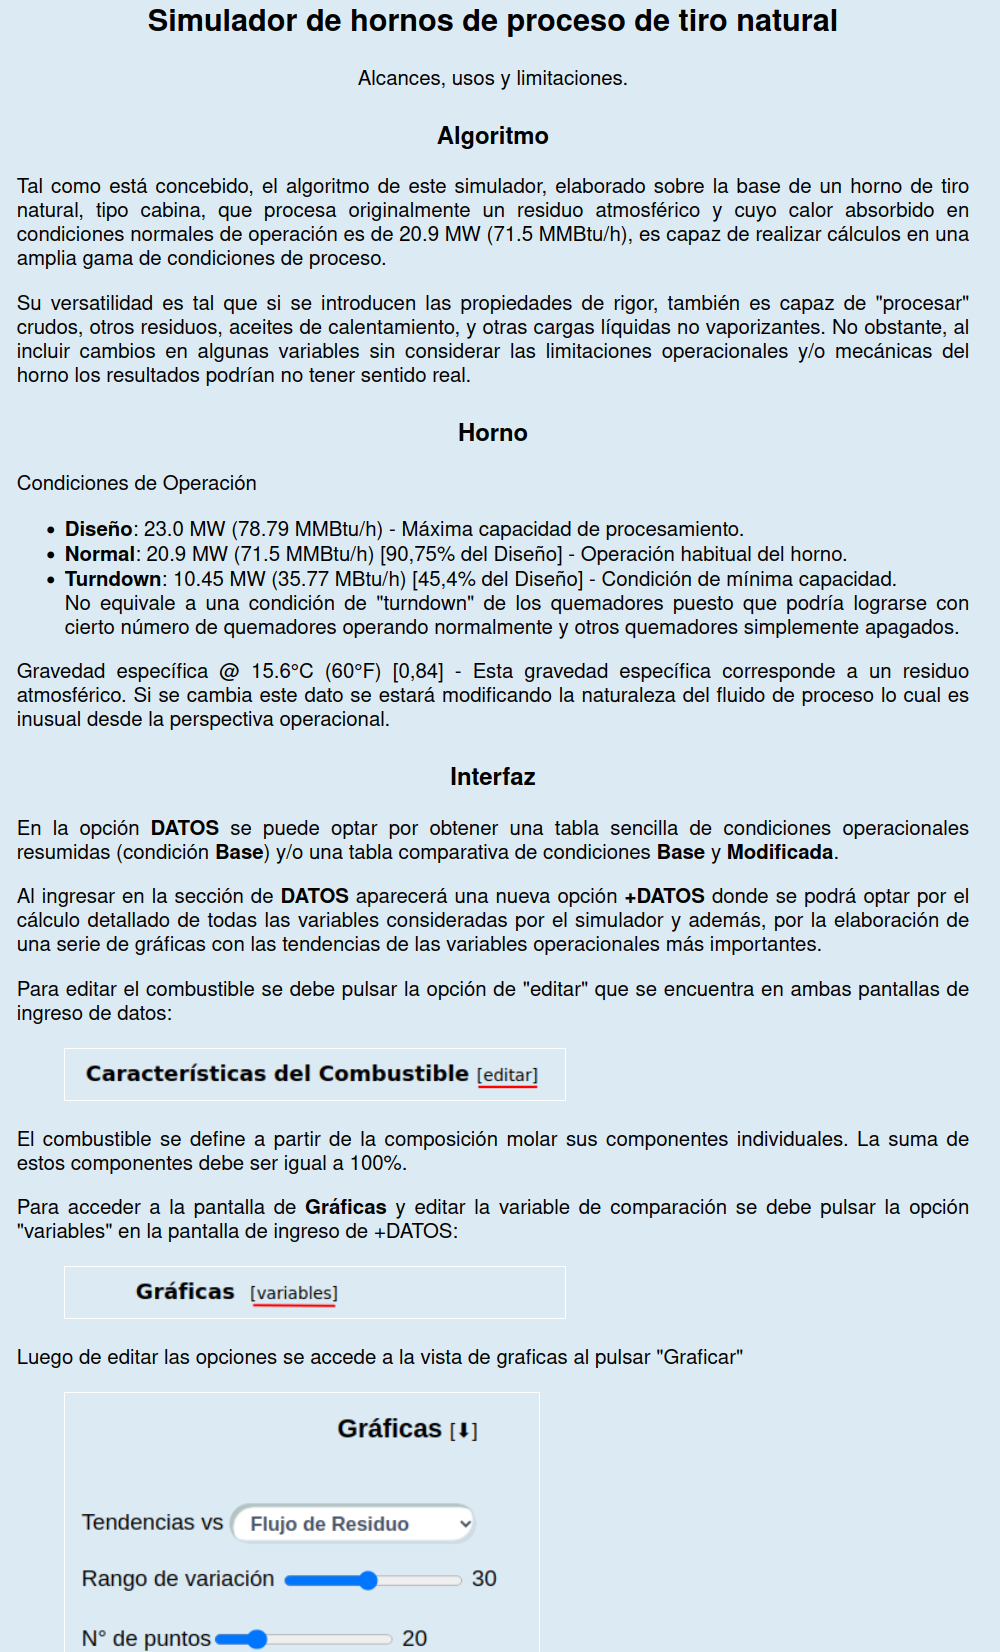
\includegraphics[scale=0.33]{images/alcance}
\caption[Página de alcances]{Referencia a página de alcances, vista introductoria a la aplicación web.}
\label{fig:alcance}
\end{center}
\end{figure}
\par La sección de usos y alcance describe como utilizar la barra de navegación del sitio web (ver Figura \ref{fig:navbar}), como editar el combustible a utilizar en las diferentes vistas de ingreso de datos y finalmente como usar la sección de gráficas o tendencias.
\begin{figure}[H]
\begin{center}

\includegraphics[scale=0.22]{images/navbar}
\caption[Barra de navegación]{Barra de navegación de la interfaz web.}
\label{fig:navbar}
\end{center}
\end{figure}

\subsubsection{Condiciones de operación de diseño mostradas}
\par En esta vista se detallan las condiciones de diseño, como se muestra a continuación:
\begin{itemize}
    \item \textbf{Diseño}: 23,0 MW (78,79 MMBtu/h) - Máxima capacidad de procesamiento recomendada.
    \item \textbf{Normal}: 20,9 MW (71,5 MMBtu/h) [90,75\% del Diseño] - Operación habitual del horno.
    \item \textbf{Turndown}*: 10,45 MW (35,77 MBtu/h) [45,4\% del Diseño] - Condición mínima de operación.
\end{itemize}
\par *No equivale a una condición de ``turndown'' de los quemadores puesto que podría lograrse con cierto número de quemadores operando normalmente y otros quemadores simplemente apagados.

\subsection{Introducción de datos}
\par En esta sección se desarrollan dos vistas:
\begin{itemize}
    \item La primera, que se accede al pulsar el botón \textbf{DATOS} en la barra de navegación, es una vista simplificada para introducir solo los datos más relevantes del proceso. Al accionar el cálculo dirige al usuario a una pantalla de resultados donde se pueden comparar dos estados de operación (ver Fig. \ref{fig:datos}).
\end{itemize}
\begin{figure}[H] \begin{center}
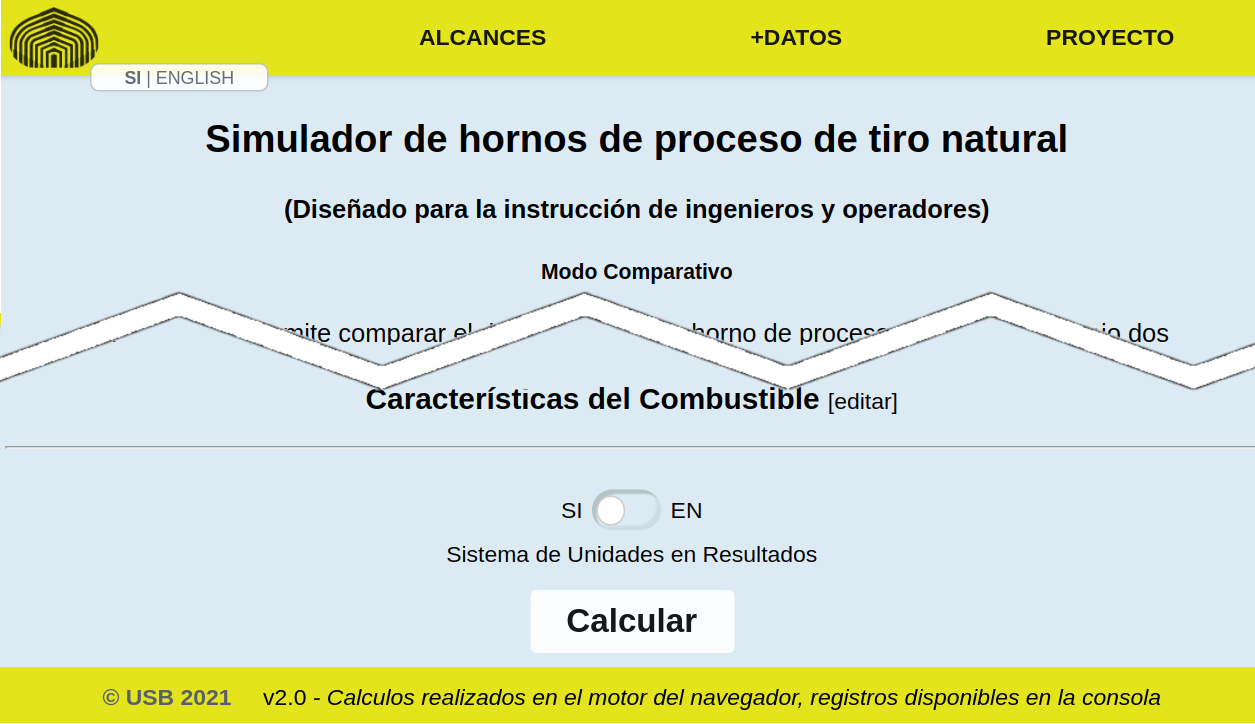
\includegraphics[scale=0.3]{images/datos}
\caption[Página de ingreso de datos para comparación]{Referencia a página de ingreso de datos utilizada para accionar el cálculo en la vista comparativa de resultados.}
\label{fig:datos} \end{center} \end{figure}
\begin{itemize}
    \item La segunda, que se accede estando en la sección de ingreso de datos simplificada al pulsar el botón \textbf{+DATOS} en la barra de navegación. En esta vista se encuentran todas las variables que permite modificar el proceso (ver Fig. \ref{fig:fulldatos}) y permite la posibilidad de accionar el cálculo para ofrecer una página de resultados extendidos. Adicionalmente se pueden accionar la generación de las curvas de tendencia escogiendo una variable a ser modificada al final de la página y pulsando el botón de graficar.
\end{itemize}
\begin{figure}[H] \begin{center}
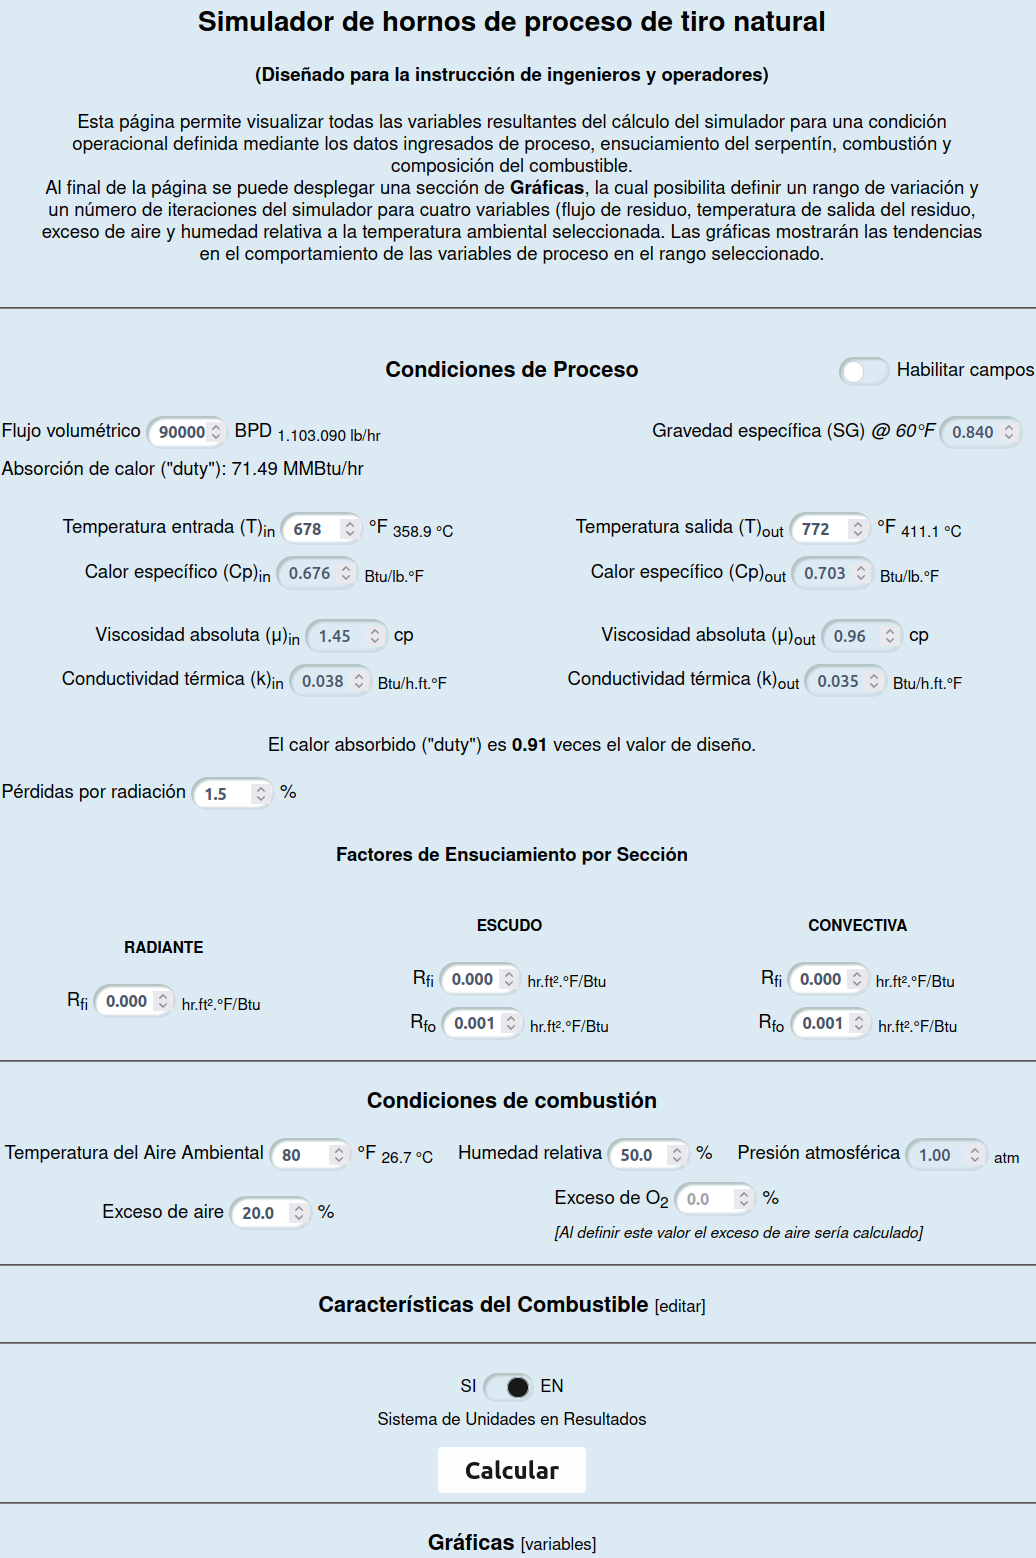
\includegraphics[scale=0.3]{images/datos2}
\caption[Página de ingreso de datos extendida]{Referencia a página de ingreso de datos extendida, con la opción de accionar la vista de resultados extendidos o la generación de gráficas de tendencia.}
\label{fig:fulldatos}
\end{center} \end{figure}
\par En ambas se puede modificar la composición molar del combustible al pulsar la opción ``editar'', como se muestra en la Figura \ref{fig:edit_fuel}:
\begin{figure}[H] \begin{center} 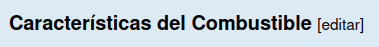
\includegraphics[scale=0.6]{images/edit_fuel}
\caption[Opción para editar el combustible]{Opción para editar el combustible al ingresar los datos.}
\label{fig:edit_fuel} \end{center} \end{figure}
\par Un ejemplo de los campos abiertos para la edición de la composición del combustible se puede apreciar en la Figura \ref{fig:edit_fuel_ext}:
\begin{figure}[hbt] \begin{center}
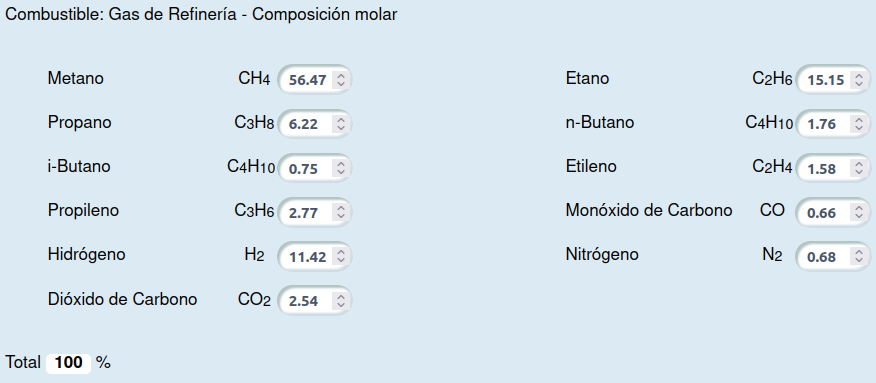
\includegraphics[scale=0.45]{images/edit_fuel_ext}
\caption[Campos para editar la composición del combustible]{Campos para editar la composición del combustible.}
\label{fig:edit_fuel_ext} \end{center} \end{figure}

\subsection{Resultados comparativos}
\par Esta vista es el resultado de accionar el cálculo en la sección de ingreso de datos simplificada. Posee el mayor potencial educativo, al resumir todas las variables resultantes y hacer una comparación entre dos condiciones de operación (Fig. \ref{fig:resultados}).
\par Aquí se pueden observar directamente los cambios en variables de interés, como los datos de ingreso, las emisiones de dióxido de carbono, el consumo de combustible, la distribución de calor dentro del horno, la temperatura de salida de los gases de combustión y la eficiencia térmica.
\par La recomendación para su uso es modificar solo una variable a la vez para su correcta interpretación.
\begin{figure}[H] \begin{center}
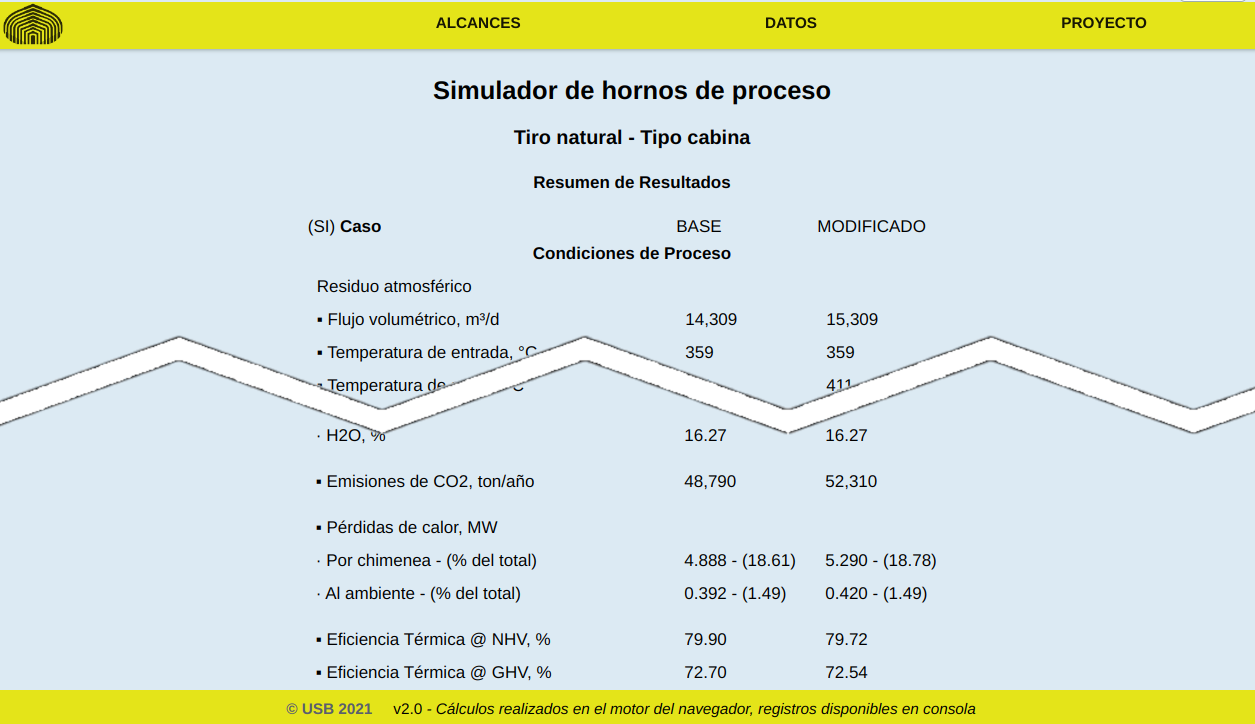
\includegraphics[scale=0.3]{images/result}
\caption[Página comparativa de resultados]
{Referencia a página comparativa de resultados, donde se pueden detallar los cambios de un estado a otro en la operación del horno.}
\label{fig:resultados} \end{center} \end{figure}

\subsection{Resultados extendidos}
\par Esta vista es el resultado de accionar el cálculo en la sección de ingreso de datos extendidos. Aquí se detallan todas las variables resultantes por cada sección del horno (Fig. \ref{fig:fullresultados}), se puede escoger el sistema de unidades a expresarse en la pantalla anterior, se uso extensamente al depurar las ecuaciones internas del algoritmo para encontrar sus puntos críticos y corregirlos.
\begin{figure}[H] \begin{center}
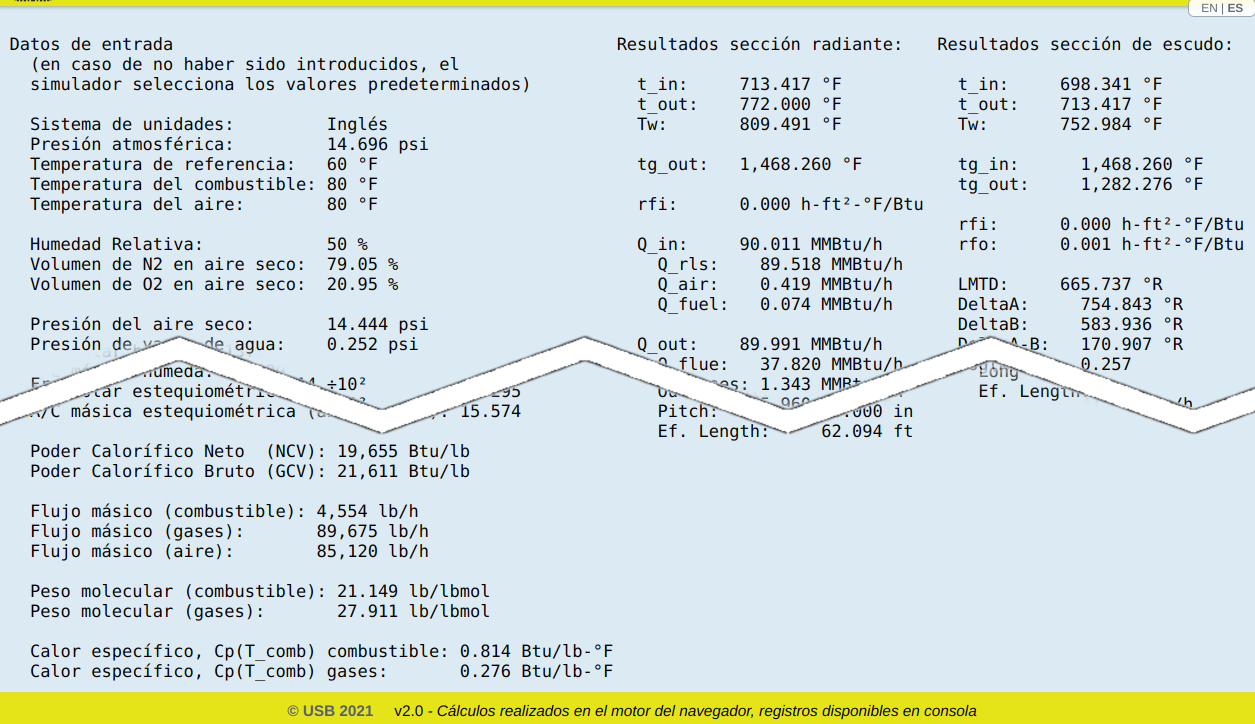
\includegraphics[scale=0.3]{images/result2}
\caption[Página extendida de resultados]{Referencia a página extendida de resultados, en ella se pueden observar a detalle las variables internas del proceso simulado.}
\label{fig:fullresultados} \end{center} \end{figure}
\par El objetivo de esta vista es tener una visión del comportamiento de todas las variables en el proceso, de aquí se pueden encontrar explicaciones no tan obvias del comportamiento de las variables finales mostradas en la vista comparativa.

\subsection{Gráficas}
\par Esta página es pensada para los usuarios más curiosos, y para futuras modificaciones del algoritmo o extensión de sus rangos (ver Figura \ref{fig:graficas}).
\begin{figure}[H]\begin{center}
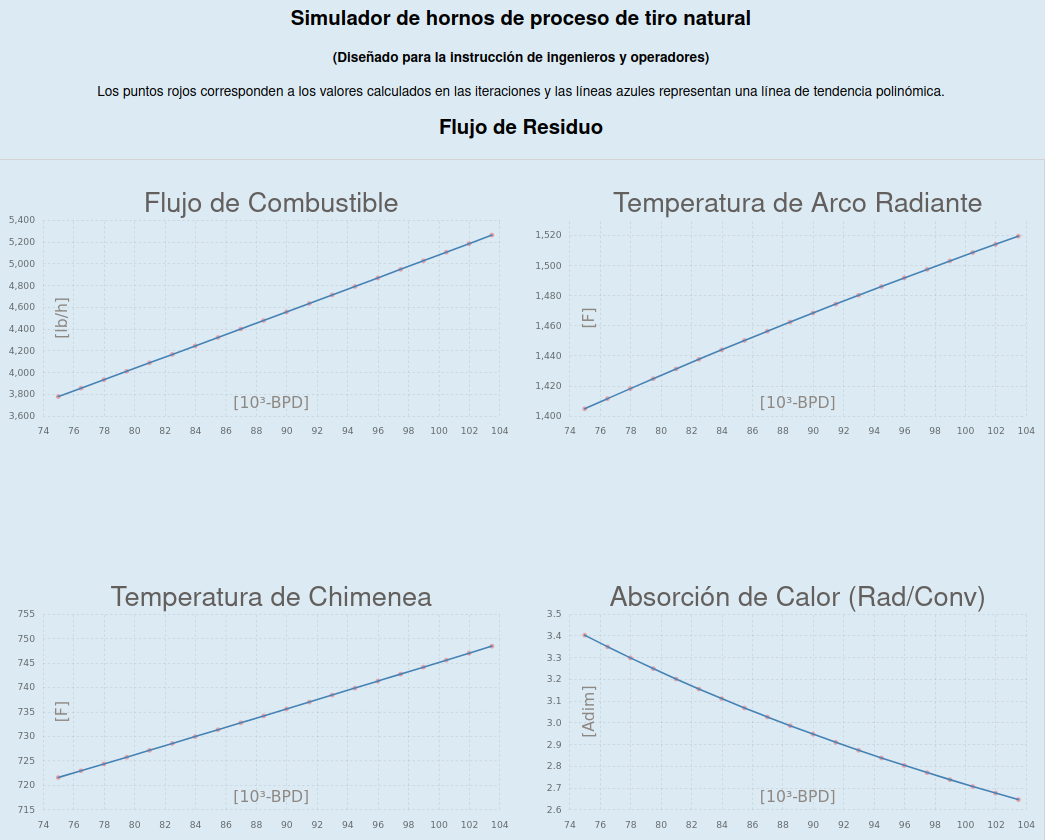
\includegraphics[scale=0.36]{images/graficas.png}
\caption[Página de gráficas]{Referencia de la página de gráficas, aquí se muestran las tendencias de las variables resultantes escogidas en el rango de variación determinado por el usuario.}
\label{fig:graficas} \end{center} \end{figure}
\par Para acceder a esta vista se debe accionar la opción de graficar ubicada al final de la página de ingreso de datos extendidos.
\par Su propósito es generar una visual del comportamiento del horno simulado a lo largo de un rango seleccionado, se usó para conseguir zonas donde los métodos aproximados del simulador no convergían y permitió sintonizar el paso, numero de iteraciones, valor inicial y tolerancia de dichos métodos.
\par En esta vista se pueden comprobar las tendencias, la continuidad y la estabilidad de las variables resultantes; también facilita la comprensión de los resultados de los fenómenos dentro del horno.

\section{Despliegue del simulador en la web}
\par En el apartado ``PROYECTO'' de la barra de navegación en la interfaz, mostrado en la Figura \ref{fig:navbar}, se puede acceder al repositorio del proyecto, ubicado en GitHub, servidor que aloja el software del simulador y lo mantiene en línea.
\par GitHub es una plataforma de alojamiento de código para el control de versiones y la colaboración. Permite trabajar de forma individual o en equipos para desarrollar proyectos con acceso desde cualquier lugar con conexión a internet.
\par Adicionalmente permite publicar sitios web estáticos, que no requieran manejo de base de datos en la nube o procesamiento de datos a nivel del servidor, para proyectos de código abierto.
\par Se usó esta ventajosa función para hacer el simulador accesible desde cualquier navegador y se encuentra disponible en el siguiente enlace: \url{https://e-usb.github.io/heater}
\par Para acceder al código alojado en GitHub se puede seguir el mismo enlace ubicado en la pestaña ``PROYECTO'' de la interfaz del simulador. \url{https://github.com/e-usb/heater}
\chapter{Uso de la clase}

\section{Sobre el uso correcto de ciertos comandos}
\subsection{Tablas}
\par Por su parte, las tablas se incluyen como usual asegurandose que la leyenda est\'e ubicada encima de la tabla. El siguiente ejemplo prodice la Tabla \ref{tbl:tabla1}.
\begin{table}
\begin{center}
\caption[T\'itulo corto]{T\'itulo largo de la tabla explicando la misma. La leyenda est\'a ubicado encima para las tablas.}
\label{tbl:tabla1}
\begin{tabular}{rcl}
\hline
Nombre & centrado & apellido\\
\hline
A & B & C \\
Gino & 4 & Lampariello \\
Judith & 6 & Del Terranova\\
\hline
\end{tabular}
\end{center}
\end{table}
\par Al hacer menci\'on a alguna tabla usar la palabra ``Tabla'' (con la primera letra en may\'uscula) seguido de la refencia a la tabla \verb+\ref{fig:tabla1}+. El \'indice de tablass deber ser incluido solamente cuando el n\'umero de tablas es superior a diez.

%\chapter{SOBRE EL USO DE ACR\'ONIMOS Y LA LISTA DE S\'IMBOLOS}
\section{Acr\'onimos}
En este cap\'itulo se describe una forma de crear los acr\'onimos compatiblemente con las normas de los decanatos. Su uso es opcional pero recomendado.  

El uso de los acronimos se hace a trav\'es del paquete {\sl acronym} (que debe ser cargado en el prea\'ambulo) y es habilitado
con el comando \verb+\useacronyms+ al principio del archivo (luego de los \'indices durante \verb+\frontmatter+). Los
acr\'onimos se definen {\em todos} en el archivo {\tt acronimos.tex} bajo el ambiente \verb+\begin{acronym}+\verb+\end{acronym}+. Para definir un acr\'onimo se usa el comando \verb+\acro{}[]{}+. La primera entrada es el nombre del acr\'onimo, la segunda entrada es el acr\'onimo propiamente y la tercera entrada es la expansi\'on del acr\'onimo. Por ejemplo, lo siguiente es el contenido del archivo \texttt{acronimos.tex} donde se crean algunas definiciones de acr\'onimos.
\begin{verbatim}
\chapter*{LISTA DE ACR\'ONIMOS}
\begin{acronym}
\acro{USB}[USB]{Universidad Sim\'on Bol\'ivar}
\acro{CCE}[Dpto.~CCE]{Departamento de C\'omputo Cient\'ifico 
     y Estad\'isitica}
\acro{DEP}[DEP]{Decanato de Estudios Profesionales}
\acro{PDF}[PDF]{Documento en Formato Portable\copyright}
\acro{PS}[PS]{PostScript\copyright}
\end{acronym}
\end{verbatim}
Una vez definidos los acr\'onimos se pueden referenciar con el comando \verb+\ac{}+ usando el nombre definido para el acr\'onimo. Por
ejemplo, \verb+\ac{USB}+ producir\'a \ac{USB}, mientras que \verb+\ac{CCE}+ producir\'a \ac{CCE}.

La clase {\sl tesis-usb} en acorde a las disposiciones del \ac{DEP}, despliega la descripci\'on
de cada acr\'onimo una sola vez cuando es referenciada la primera vez en cada cap\'itulo. Todo
los usos sucesivos no son expandidos, por ejemplo:

\noindent \verb+\ac{LI}+$\rightarrow$ \ac{LI}\\
\verb+\ac{LI}+$\rightarrow$ \ac{LI}\\
\verb+\ac{LI}+$\rightarrow$ \ac{LI}\\
\verb+\ac{LI}+$\rightarrow$ \ac{LI}\\
\verb+\ac{CCE}+$\rightarrow$ \ac{CCE}

Nota: Si el comando \verb+\useacronyms+ est\'a comentado al principio de {\tt main.tex} y se
usan acr\'onimos a lo largo del libro, estos no van a funcionar resultando en errores de compilación.

\section{Lista de s\'imbolos}
La lista de s\'imbolos o notaci\'on matem\'atica se recomienda hacer manualmente. Por ejemplo, se puede incluir el siguiente c\'odigo luego de los \'indices.
\begin{verbatim}
\chapter*{Notaci\'on matem\'atica}
\begin{tabular}{ll}
$\mathbb{R}$ & Conjunto de n\'umeros reales\\
$M_{m,n}$ & Espacio de las matrices de tama\~no $m$ por 
     $n$ con entradas reales\\
$\mathcal{L}$ & Operador de Laplace\\
$\emptyset$ & Conjunto vac\'io
\end{tabular}
\end{verbatim}
%\chapter{DE C\'OMO COMPILAR EL LIBRO}

\chapter*{Conclusiones}

%\begin{itemize}
    %\item 
    \par Se desarrollo exitosamente un modelo capaz de simular la operación de hornos de proceso, enfocado al adiestramiento de ingenieros y operadores, y con el objetivo de aumentar la eficiencia de estos equipos para disminuir el consumo de combustibles fósiles y generar menos gases de efecto invernadero.

    %\item 
    \par El modelo integra las ecuaciones de transferencia de calor y conservación de masa y energía en un algoritmo que simula el comportamiento estacionario de un horno de fuego directo, se comprobó su capacidad para generar resultados estables y confiables de las variables de proceso establecidas.
    
    %\item 
    \par El simulador para adiestramiento de hornos de proceso es una herramienta computacional de disposición pública y de código abierto, escrita en el lenguaje de programación JavaScript, que refiere parámetros confiables y prácticos para el uso académico o industrial dentro de las características mecánicas establecidas. El acceso directo se encuentra siguiendo el enlace (\url{https://e-usb.github.io/heater}).
    
    %\item 
    \par Los resultados generados por el simulador fueron validados aceptablemente mediante su comparación con un software comercial empleado para el diseño y evaluación termomecánica de hornos de proceso. Las tendencias de las variables operacionales simuladas mostraron resultados totalmente coherentes con la operación real de estos hornos en refinerías y plantas petroquímicas.

    %\item 
    \par Se incrementó el alcance del algoritmo desarrollado con la implementación de un modo comparativo y un modo de visualización de tendencias, aumentando las opciones de los usuarios al interactuar con el simulador.
%\end{itemize}
\nocite{*}
\bibliography{referencias}
\appendix
\chapter{Métodos iterativos}\label{apx:met}

\par En matemática computacional, un método iterativo trata de resolver un problema (como una ecuación o un sistema de ecuaciones) mediante aproximaciones sucesivas a la solución, empezando desde una estimación inicial. Esta aproximación contrasta con los métodos directos, que tratan de resolver el problema en un único intento (como resolver un sistema de ecuaciones Ax=b encontrando la inversa de la matriz A).
\par A modo de referencia se describen los métodos de aproximación de utilizados a continuación.

\section{Newton Raphson}
\par Es un algoritmo para encontrar aproximaciones de los valores iguales a ceros, o raíces, para una función de números reales. También puede ser usado para encontrar el máximo o mínimo de una función real, encontrando los puntos de inflexión, donde se iguala a cero su primera derivada, pero nuestro caso de enfoque será el mencionado inicialmente.
\par El método de Newton es un método abierto, en el sentido de que no está garantizada su convergencia global. La única manera de alcanzar la convergencia es seleccionar un valor inicial (semilla) lo suficientemente cercano a la raíz de la función buscada. Así, se ha de comenzar la iteración con un valor razonablemente cercano al cero (también denominado punto de arranque o valor supuesto). La relativa cercanía del punto inicial a la raíz depende mucho de la naturaleza de la propia función; si ésta presenta múltiples puntos de inflexión o pendientes grandes en el entorno de la raíz, entonces las probabilidades de que el algoritmo diverja aumentan, lo cual exige seleccionar un valor supuesto cercano a la raíz. Una vez que se ha hecho esto, el método linealiza la función por la recta tangente en ese valor supuesto. La abscisa en el origen de dicha recta será, según el método, una mejor aproximación de la raíz que el valor anterior. Se realizarán sucesivas iteraciones hasta que el método haya convergido a la tolerancia deseada o se alcanza el numero límite de iteraciones. 
\par Así como el valor inicial, el paso de cada iteración y la tolerancia, todas son variables que se ajustan a conveniencia en este método; los rangos de operación alcanzados por el simulador del horno dependerán en gran medida de estos valores.
\par El método se basa en el desarrollo de Taylor de la función cuya raíz se quiere calcular. Al considerar la ecuación $f(x)=0$, y suponiendo que posee una y sólo una solución $\alpha\in[a,b]$. Se parte de un punto $x_0$ suficientemente cercano a dicha raíz, se escribe:
\begin{equation*}
f(\alpha) = f(x_0)
    + (\alpha-x_0)f^\prime(x_0) 
    + \frac{\alpha-x_0}{2}f^{\prime\prime}(x_0+\theta h)
\end{equation*}
\par con $0<\theta<1$, $h=\alpha-x_0$.
\par Si se supone que $f^\prime(x)$ no se anula en $[a,b]$, y que la diferencia $\alpha-x_0$ es muy pequeña, el método de Newton-Raphson consiste en despreciar el sumando en $(\alpha-x_0)/2$ del desarrollo anterior, quedando con la aproximación:
\begin{equation*}
f(\alpha) \approx f(x_0) + (\alpha-x_0)f^\prime(x_0)
\end{equation*}
\par Como $\alpha$ es la solución de la ecuación $f(x)=0$, se tiene que $f(\alpha)=0$ y por tanto, de la expresión anterior se sigue que:
\begin{equation*}
f(x_0)+(\alpha-x_0)f^\prime(x_0) \approx 0
\end{equation*}
\par y despejando $\alpha$ resulta:
\begin{equation*}
\alpha \approx x_0 - f(x_0)f^\prime(x_0) = x_1
\end{equation*}
\par La implementación usada puede verse en los anexos donde se encuentra el código fuente del simulador.

\section{Bisección}
\par Se basa en el teorema del valor intermedio (TVI), el cual establece que toda función continua $f$ en un intervalo cerrado $[a,b]$ toma todos los valores que se hallan entre $f(a)$ y $f(b)$. Esto es que todo valor entre $f(a)$ y $f(b)$ es la imagen de al menos un valor en el intervalo $[a,b]$. En caso de que $f(a)$ y $f(b)$ tengan signos opuestos, el valor cero sería un valor intermedio entre $f(a)$ y $f(b)$, por lo que con certeza existe un  $p\in [a,b]$ que cumple  $f(p)=0$. De esta forma, se asegura la existencia de al menos una solución de la ecuación $f(x)=0$.
\par Es también un algoritmo de búsqueda de raíces o ceros en funciones reales, que trabaja dividiendo un intervalo dado a la mitad y seleccionando el subintervalo que tiene la raíz. Suele requerir más iteraciones para alcanzar la tolerancia deseada que el método Newton Raphson descrito anteriormente, además de conocer de antemano el intervalo donde se encuentra la raíz deseada, su ventaja es que en funciones continuas se puede garantizar su convergencia.
\chapter{EJEMPLO DE IMAGEN EN APÉNDICE}\label{apx:img}
\begin{figure}[ht]
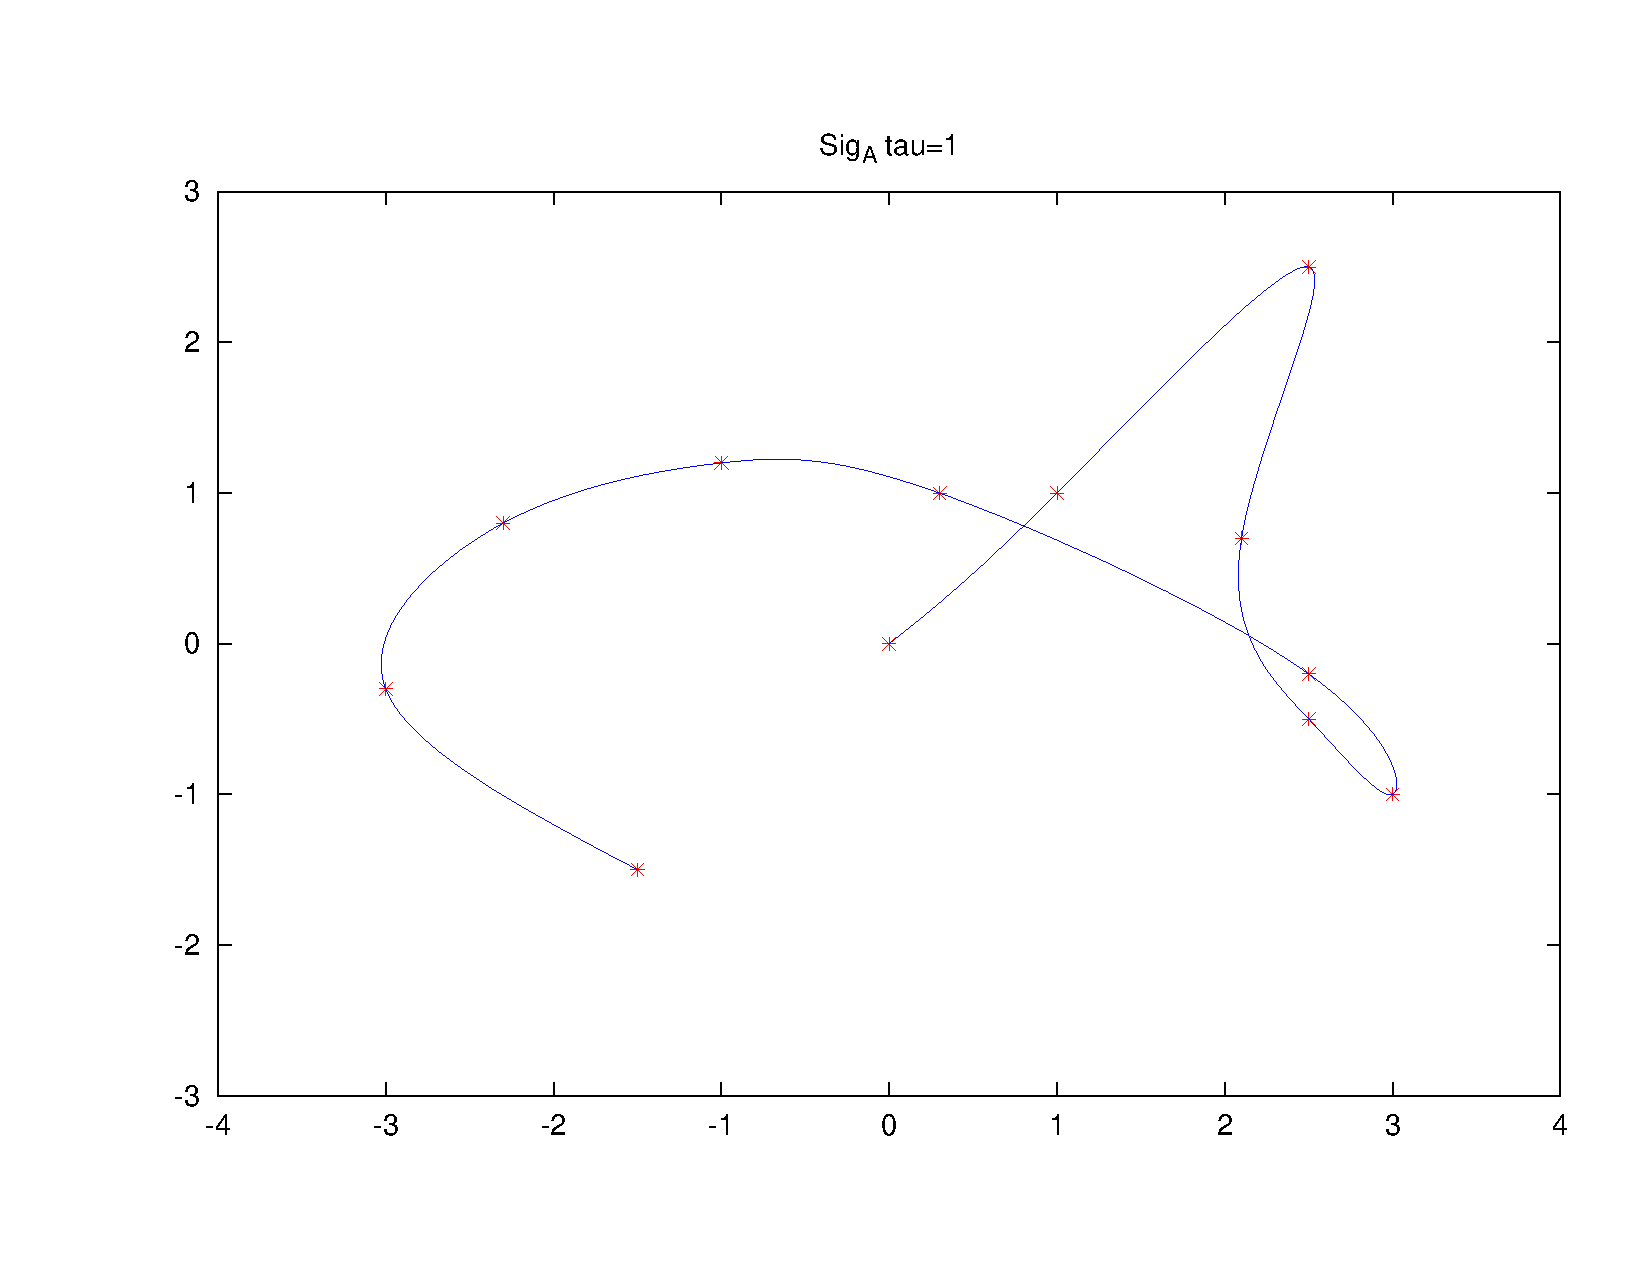
\includegraphics[scale=0.48,angle=0]{images/ejemplo}
\caption[Título corto de imagen]{Título corto de imagen}\label{img:imgscl}
\end{figure}




\end{document}
